\section{Conclusions.}
In the literature, we found statistical studies proving that twinning is an inherently stochastic phenomenon distributed probabilistically across geometrical parameters. Previous deterministic models failed to capture this stochastic nature adequately. We addressed this limitation by modeling the stochasticity in our constitutive law using a random sampling technique inspired by Monte Carlo methods.  For simplicity, we consider the random sampling to be uniformly distributed, and we control the frequency of sampling and the range of random numbers.

\vspace{0.2cm}

Based on experimental observations and results from energy-based modeling approaches, we assume that the nucleation of twins occurs at grain boundaries. We employ selective random sampling at grain boundaries to model the nucleation events, using local stress criteria. For twin growth, which includes propagation and band thickening, we use selective random sampling of neighboring twinned voxels/elements, as a newly nucleated site induces large shear in the neighborhood. The distribution of random numbers and frequency control can be applied separately for nucleation and growth events.

\vspace{0.2cm}

Next, we model twinning as a discrete entity, enabling a spatially resolved representation of twinning events that aligns with experimental observations. This approach allows for more accurate prediction of texture evolution, which volume fraction-based models lack the capability to resolve spatially.

\vspace{0.2cm}

We consider twinning as a ``Jump" rather than a ``pseudo-slip" approach, applying the twinning shear and reorientation directly to the plastic deformation gradient $F_p$. This captures the localized deformation effects of twinning at appropriate time scales. For this, we use the correspondence matrix approach, providing a rigorous crystallographic basis by combining the twinning shear (S) and lattice rotation (U) of mechanical twinning to model the lattice reorientation and deformation associated with twinning.

\vspace{0.2cm}

For implementing our model, we chose DAMASK, an open-source crystal plasticity software that provides the facility to modify constitutive laws and integrate custom formulations due to its modular construction. DAMASK's ability to access internal subroutines facilitated the implementation of our model on a stable platform for testing. We treat twinning as an intermediate configuration with a sudden jump in the plastic deformation gradient $F_p$, departing from the gradual $F_p$ rate evolution associated with dislocation slip in crystal plasticity. This is implemented by modifying the time integration algorithm for kinematic variables in DAMASK and circumventing loops for convergence while updating the plastic deformation gradient.

\vspace{0.2cm}

Our work advances the understanding and modeling of deformation twinning in HCP metals by addressing gaps or limitations identified in the literature, such as the stochastic nature of twinning, accurate spatial resolution of twins, and capturing the localized deformation effects through a crystallographically rigorous approach. This can potentially lead to more accurate predictions of texture evolution and deformation behavior in HCP metals, enabling better material design and performance optimization.

\section{Future scope: Full Scale Model Testing.}
For publication of the discrete twinning constitutive model it is necessary to test it against other models and with experiments. We need to run simulations for 3D polycrystal Representative Volume Elements (RVEs) for running these tests. Here we discuss the process of model testing.

\subsection{Benchmark the simulations.}

Before running polycrystal simulations to test our code, it is essential to benchmark the simulation results against known solutions or experimental data. This process involves running a set of pre-processing codes with well-understood material parameters and boundary conditions and comparing the simulation results with established benchmarks. For this purpose, we have chosen to benchmark our simulations against the results of Wang et al. (2014) \cite{WANG201477}, where simulations were performed on pure magnesium using the DAMASK software, and the results were compared with experimental observations.

Benchmarking against a reliable source serves several purposes:

\begin{enumerate}
    \item Verification: It verifies the correct implementation of the constitutive model, numerical algorithms, and boundary conditions within our code.
    \item Validation: It validates the model's ability to reproduce known phenomena and results accurately.
    \item Calibration: It aids in calibrating material parameters and identifying potential discrepancies or sources of error.
    \item Establishing Confidence: Successful benchmarking builds confidence in the reliability and accuracy of our simulation framework before proceeding with further investigations or parametric studies.
\end{enumerate}

\subsection{Benchmark simulation setup.}

Lattice parameters and elastic properties of Mg for the simulation is based on \cite{HULL1922189}  \\ $\{\bar{1} 0 1 2\} \langle 1 0 \bar{1} 1 \rangle$ Extension twin system in Magnesium:

\begin{table}[H]
    \begin{subtable}{0.45\textwidth}
    \centering
    \caption{Crystallography of twinning.}
    \label{tab:Twin_geometry}
        \begin{tabular}{cccc}
        \hline
        $\nu_1$ & $K_1$ & $\nu_2$ & $K_2$ \\
        \hline
        $\langle  \bar{1} 0 1 1 \rangle$ & $\{ 1 0 \bar{1} 2 \}$ & $\langle 1 0 \bar{1} 1 \rangle$ & $\{ 1 0 \bar{1} \bar{2} \}$ \\
        \hline
        \end{tabular}
    \end{subtable}
    \begin{subtable}{0.45\textwidth}
    \centering
    \caption{Lattice parameters.}
    \label{tab:cOverA}
        \begin{tabular}{cccc}
        \hline
        parameter & c & a & c/a \\
        \hline
        value & 1.6235 & 1 & 1.6235 \\
        \hline
        \end{tabular}
    \end{subtable}
    \caption{Crystallography of twinning and lattice parameters.}
    \label{tab:Twin_crystallography}
    
\end{table}



%next subtables should start immediately after previous one else it will not be side by side.
\begin{table}[H]

    \begin{minipage}[h]{0.45\textwidth}
    \begin{subtable}{\textwidth}
    \centering
    \caption{$\langle \Bar{1} 0 1 1 \rangle \{ 1 0 \Bar{1} 2 \}$ extension twin system.}
    \label{tab:Twins1}
        \begin{tabular}{ccc}
            \hline
            index & plane normal & slip direction \\
            \hline
            $V1$ & $(\bar{1} 1 0 2)$ & $[ 1 \bar{1} 0 1]$ \\
            $V2$ & $(1 0 \bar{1} 2)$ & $[ \bar{1} 0 1 1]$ \\
            $V3$ & $(0 \bar{1} 1 2)$ & $[ 0 1 \bar{1} 1]$ \\
            $V4$ & $(1 \bar{1} 0 2)$ & $[ \bar{1} 1 0 1]$ \\
            $V5$ & $(\bar{1} 0 1 2)$ & $[ 1 0 \bar{1} 1]$ \\
            $V6$ & $(0 1 \bar{1} 2)$ & $[ 0 \bar{1} 1 1]$ \\
            \hline
        \end{tabular}
    \end{subtable} 
    \begin{subtable}{\textwidth}
    \centering
    \caption{$\langle 2 \bar{1} \bar{1} 0 \rangle \{ 0 0  0 1 \}$ basal slip system.}
    \label{tab:Slips0}
        \begin{tabular}{ccc}
            \hline
            index & plane normal & slip direction \\
            \hline
            $1$ & $(0 0 0 1)$ & $[ 2 \bar{1} \bar{1} 0]$ \\
            $2$ & $(0 0 0 1)$ & $[ \bar{1} 2 \bar{1} 0]$ \\
            $3$ & $(0 0 0 1)$ & $[ \bar{1} \bar{1} 2 0]$ \\
            \hline
        \end{tabular}
    \end{subtable} 
    \begin{subtable}{\textwidth}
    \centering
    \caption{$\langle 2 \bar{1} \bar{1} 0 \rangle \{ 0 1 \bar{1} 0 \}$ prismatic slip system.}
    \label{tab:Slips1}
        \begin{tabular}{ccc}
            \hline
            index & plane normal & slip direction \\
            \hline
            $1$ & $(0 \bar{1} \bar{1} 0)$ & $[ 2 \bar{1} \bar{1} 0]$ \\
            $2$ & $(\bar{1} 0 0 1)$ & $[ \bar{1} 2 \bar{1} 0]$ \\
            $3$ & $(1 \bar{1} 0 0)$ & $[ \bar{1} \bar{1} 2 0]$ \\
            \hline
        \end{tabular}
    \end{subtable}    
    \end{minipage}%  
    \hfill
    \begin{minipage}[t]{0.45\textwidth}
    \begin{subtable}{\textwidth}
    \centering
    \caption{$\langle 2 \bar{1} \bar{1} 0 \rangle \{ 0 1 \Bar{1} 1 \}$ 1st  order pyramidal slip system.}
    \label{tab:Slips2}
        \begin{tabular}{ccc}
            \hline
            index & plane normal & slip direction \\
            \hline
            $V1$ & $(0 1 \bar{1} 1)$ & $[ 2 \bar{1} \bar{1} 0]$ \\
            $V2$ & $(\bar{1} 0 1 1)$ & $[ \bar{1} 2 \bar{1} 0]$ \\
            $V3$ & $(1 \bar{1} 0 1)$ & $[ \bar{1} \bar{1} 2 0]$ \\
            $V4$ & $(\bar{1} 1 0 1)$ & $[ 1 1 \bar{2} 0]$ \\
            $V5$ & $(0 \bar{1} 1 1)$ & $[ \bar{2} 1 1 0]$ \\
            $V6$ & $(1 0 \bar{1} 1)$ & $[ 1 \bar{2} 1 0]$ \\
            \hline
        \end{tabular}
    \end{subtable} 
    \begin{subtable}{\textwidth}
    \centering
    \caption{$\langle 2 \bar{1} \bar{1} 3 \rangle \{ \bar{2} 1 1 2\}$ 2nd  order pyramidal slip system.}
    \label{tab:Slips3}
        \begin{tabular}{ccc}
            \hline
            index & plane normal & slip direction \\
            \hline
            $V1$ & $(\bar{2} 1 1 2)$ & $[ 2 \bar{1} \bar{1} 3]$ \\
            $V2$ & $(1 \bar{2} 1 2)$ & $[ \bar{1} 2 \bar{1} 3]$ \\
            $V3$ & $(1 1 \bar{2} 2)$ & $[ \bar{1} \bar{1} 2 3]$ \\
            $V4$ & $(2 \bar{1} \bar{1} 2)$ & $[ \bar{2} 1 1 3]$ \\
            $V5$ & $(\bar{1} 2 \bar{1} 2)$ & $[ 1 \bar{2} 1 3]$ \\
            $V6$ & $(\bar{1} \bar{1} 2 2)$ & $[ 1 1 \bar{2} 3]$ \\
            \hline
        \end{tabular}
    \end{subtable}
    \end{minipage}
    \caption{Slip and twin systems.}
    \label{tab:Crystallography}
    
\end{table}

Table \ref{tab:Mat_properties} from \cite{Tromans2011ELASTICAO} \cite{AGNEW20064841} are the material parameters of Mg where $\xi_0$ $\xi_\infty$ values are initial and bounding Critical Resolved Shear Stress for various slip and twin systems. $h_0$ values are system dependent fitting parameters.


\begin{table}[H]
    \begin{subtable}[h]{0.45\textwidth}
    \centering
    \caption{Deformation twinning parameters.}
    \label{tab:Twin_parameters}
          \begin{tabular}{lS[table-format=4.1]l}
                \hline
                property & {value} & unit \\
                \hline
                 $\xi_{0,T1}$ & 40.0 & MPa \\
                 $h^{tw-tw}_{0}$ & 50.0 & MPa \\
                 $h^{tw-s}_{0}$ & 150.0 & MPa \\
                \hline
          \end{tabular}
    \end{subtable}
    \vspace{-2em}
    
    \begin{subtable}[h]{0.45\textwidth}
    \centering
    \caption{Elastic Properties}
    \label{tab:Elastic_properties}
         \begin{tabular}{l S[table-format=4.1] l}
         \hline
          property & {value} & unit \\
          \hline
          $C_{11}$ & 59.3 & GPa \\
          $C_{33}$ & 61.5 & GPa \\
          $C_{44}$ & 16.4 & GPa \\
          $C_{12}$ & 25.7 & GPa \\
          $C_{13}$ & 21.4 & GPa \\
          \hline
          \end{tabular}
    \end{subtable}
    \begin{subtable}[h]{0.45\textwidth}
    \centering
    \caption{Dislocation slip parameters.}
    \label{tab:Slip_parameters}
          \begin{tabular}{l S[table-format=4.1] l}
                \hline
                property & {value} & unit \\
                \hline
                $\xi_{0,basal}$ & 10.0 & MPa \\
                $\xi_{\infty,basal}$ & 40.0 & MPa \\
                $\xi_{0,prism}$ & 55.0 & MPa \\
                $\xi_{\infty,prism}$ & 135.0 & MPa \\
                $\xi_{0,pyr\langle a\rangle}$ & 60.0 & MPa \\
                $\xi_{\infty,pyr\langle a\rangle}$ & 150.0 & MPa \\
                $\xi_{0,pyr\langle c+a\rangle}$ & 60.0 & MPa \\
                $\xi_{\infty,pyr\langle c+a\rangle}$ & 150.0 & MPa \\
                $h^{s-s}_{0}$ & 500.0 & MPa \\
                $h^{s-tw}_{0}$ & 0.0 & MPa \\
                \hline
          \end{tabular}
    \end{subtable}

    
\caption{Material parameters of magnesium used for simulations.}
\label{tab:Mat_properties}

\end{table}

The figure \ref{Benchmark_simulation} shows a benchmark simulation result for Pure Mg poly-crystal with 20 randomly oriented grains under subjected to shear in XY direction with below boundary condition:
\begin{equation}
    \dot{F} = \begin{bmatrix}  0 & 10^{-3} & 0 \\ 0 & 0 & 0 \\  0 & 0 & 0 \end{bmatrix}
\end{equation}

\begin{figure}[H]
    \centering
    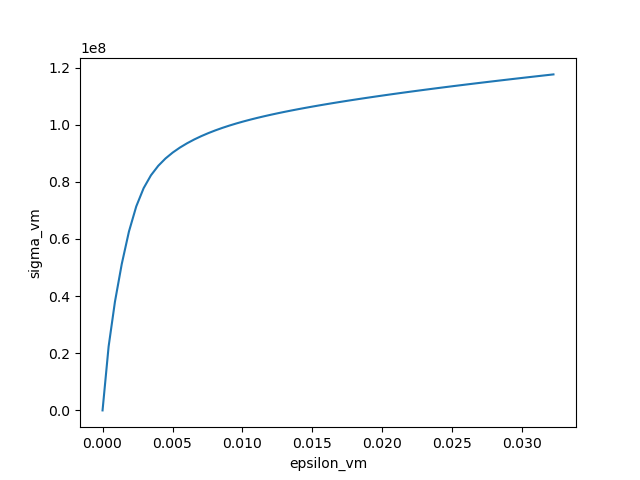
\includegraphics[width=0.5\textwidth]{images/plot.png}
    \caption{von Mises Equivalent stress-strain curve for pure Mg under shear.}
    \label{Benchmark_simulation}
\end{figure}


%\subsection{Comparison study with previous models.}
%Once the benchmark is chosen we apply it to test our model and we also use it to test our model with previous models.

%\subsubsection{Parametric studies on the model}
%In the final stage we carry out parametric studies of our model with experimental results.

\subsection{Comparison of Different Constitutive Models.}
It is essential to compare the computational efficiency and prediction capability of different constitutive models to assess their relative strengths and limitations. Since the MTech project spanning one year was dedicated to developing the constitutive model, comparative studies and analysis can be conducted as an extension of this work.

\subsection{Computational Efficiency.}
The computational effort required to generate the results can be compared across different models. For a fair comparison, the same inputs should be used to run the simulations, including the representative volume element, material parameters, and boundary conditions. Since the development of our model focused on computational efficiency, assessing its performance in this aspect will be a crucial future scope of this research work.

\subsection{Prediction capability.}
Our current model predicts the spatial evolution of twinning as a discrete quantity, which is physically accurate. In other words, our model predicts the texture evolution resulting from deformation twinning. It is also possible to compare other parameters, such as the load-deformation response, from different models and with experimental results to evaluate their predictive capabilities.

\subsection{Parametric Study of the model results.}
The influence of various parameters, including texture, grain size, grain morphology, strain rate, and loading conditions, on deformation twinning can be studied using the results of the model. These results can be compared with experimental data to validate the model's ability to capture the effects of different parameters accurately.

\subsection{Validation and Verification.}
It is crucial to validate and verify the constitutive model by comparing its predictions with experimental observations and established theoretical frameworks. This process involves assessing the model's ability to reproduce known phenomena accurately and ensuring that its underlying assumptions and formulations are consistent with fundamental principles.

\section{Future Scope: Implementation in ABAQUS as UMat.}
While DAMASK provides a basic finite element solver, a future implementation of the discrete twinning model can be made as a user-defined material (UMAT) in the ABAQUS finite element software. ABAQUS is a widely used and well-established commercial software package for finite element analysis, offering several advantages for the implementation and deployment of advanced constitutive models.




\subsection{ABAQUS Software:}
Robust and Stable Solvers: ABAQUS offers implicit finite element solvers renowned for their numerical stability and convergence properties, enabling the accurate simulation of complex material behavior and large deformations.

\begin{itemize}
    \item \textbf{User-Defined Material Capabilities:} ABAQUS allows users to implement custom constitutive models through UMATs, providing a flexible framework for incorporating advanced material models into simulations.
    \item \textbf{Pre- and Post-Processing Tools:} ABAQUS includes comprehensive pre-processing tools for model generation, mesh generation, and boundary condition assignment, as well as post-processing tools for visualizing and analyzing simulation results.
\end{itemize}

\subsection{Advantages of the Finite Element Method (FEM):}

\begin{itemize}
    \item \textbf{Complex Alloy System Modeling:} FEM can handle complex alloy systems where microstructural features such as precipitates, phases, and grains with complex morphologies can be accurately modeled into the Representative Volume Element (RVE) and discretized using tetrahedral or hexahedral elements.
    \item \textbf{Accurate Representation of Geometry and Boundary Conditions:} FEM allows for the precise representation of complex geometries and the application of a wide range of boundary conditions, enabling realistic simulations of actual engineering components and structures.
    \item \textbf{Adaptive Mesh Refinement:} Advanced FEM solvers like ABAQUS offer adaptive mesh refinement capabilities, which can automatically refine the mesh in regions of high deformation gradients or stress concentrations, improving the accuracy of the solution while optimizing computational resources.
\end{itemize}

\subsection{Additional Advantages: Wide Industry Adoption: }

ABAQUS is widely adopted across various industries, including automotive, aerospace, and manufacturing, ensuring compatibility with industry-standard practices and facilitating knowledge transfer and collaboration.


 %${https://petsc.org/release/overview/integrator_table/}$
 %$https://mooseframework.inl.gov/syntax/Executioner/TimeIntegrator/$
 % https://mooseframework.inl.gov/source/materials/crystal_plasticity/FiniteStrainUObasedCP.html
 % https://mooseframework.inl.gov/source/materials/crystal_plasticity/ComputeMultipleCrystalPlasticityStress.html
 % https://www.dropbox.com/s/23wj304q5rnjrtd/WARP3D_Intro_Lecture.pdf?e=1&dl=0